\subsection{Communications}
The satellite communication system will consist of a single patch antenna (Figure \ref{fig:comms} a) set in the S band at 2.2GHz frequency and BPSK modulation. Given the wide signal spread of the antenna and the fact that the proposed ground station (Figure \ref{fig:comms} b) receiver is well within close proximity to the target area. The satellite will not have to adjust orientation to transmit data or receive instructions.

The antenna is expected to transmit no more than 3 images per pass, 2 of which have an average size of $4MB$ and one infrared image with a size of $2.5MB$. Given that the average access time with the ground station is 15 minutes, a signal bandwidth of $1Mbps$ was selected. With the selected antenna characteristics, the communication system power requirement is estimated at $1.5W$.\\
\begin{table}[hbt!]
\centering
\caption{Communications Table}
\begin{tabular}{lll}
\rowcolor[HTML]{C0C0C0} 
Parameter             & Value & Units \\ \hline
Power                 & 1.5   & W     \\
Line loss             & -3    & dB    \\
Frequency             & 2.29  & GHz   \\
Transmitter gain      & 6.5   & dB    \\
Atmospheric losses    & -0.99 & dB    \\
Receiver gain         & 36    & dB    \\
Operating temperature & 260   & K     \\
Bit rate              & 1     & Mbps  \\
Link budget           & 27.02 & dB    \\
Link margin           & 16.25 & dB   
\end{tabular}
\label{Tab:comms}
\end{table}
\\
\begin{figure}[hbt!]
    \centering
    \subfloat[Cubesat Path Antenna]{{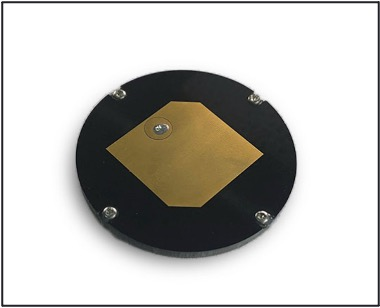
\includegraphics[width=7cm, scale=0.8]{Images/c1.jpg} }}\label{fig:c1}
    \qquad
    \subfloat[Ground Station Receiver]{{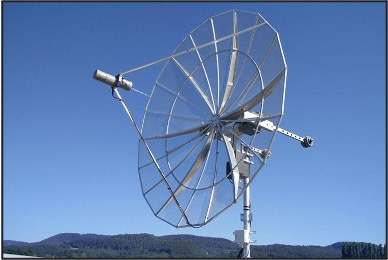
\includegraphics[width=7cm]{Images/c2.jpg} }}\label{fig:c2}
    \caption{Communication Mechanism}
    \label{fig:comms}
\end{figure}

\subsection{Command and Data Handling}
Data handling will be managed by the ARM Cortex on board compared manufactured by EnduoSat \cite{Endurosat}. This command and control computer shown in Figure \ref{fig:obc} has an excellent M7 processor that provides many great features at an estimated cost of \$10,000. This includes an ARM Cortex M7 processor and a 2 MB of memory for caching. Additionally the computer offers a built-in clock, 3-axis magnetometer, and MicroSD card slots (see Table \ref{Tab:obc}). Finally the computer has many interfaces including 4x RS-485, 2x RS-422, 3x UART, 2x I2C, SPI, USB, and CAN. These features allow for Hurrisat to manage all of its computing requirements and stay within the power budget requirements.

\begin{table}[hbt!]
\centering
\caption{OBC Data Handling}
\label{Tab:obc}
\begin{tabular}{lcl}
\rowcolor[HTML]{C0C0C0} 
\textbf{Parameter}                                                           & \multicolumn{1}{l}{\cellcolor[HTML]{C0C0C0}\textbf{Value}} & \textbf{Units} \\
Processor         & ARM Cortex M7   & N/A            \\
Program Memory         & 2     & MB             \\
Storage expansion slot & MicroSD    & 8-bit pin up to 32GB \\
SRAM & 1                                                          & MB             \\
External FRAM Memory    & 8   & Mbit           \\
Mass & 130                                     & g              \\
Interfaces & 2x RS-422, 3x  UART,SPI, USB, CAN &  N/A
\end{tabular}
\end{table}\\[.2in]

\begin{figure}[hbt!]
    \vspace{5mm}
    \centering
    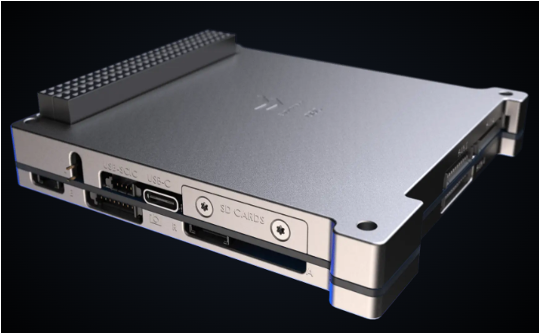
\includegraphics[width=\textwidth,frame,height=6cm]{Images/obc.png}
    \caption{On Board Computer}
    \label{fig:obc}
\end{figure}
\subsection{Electrical}
The average power drawn throughout the mission is approximately $47.8W$, which is a reasonable power requirement for a 6U cubesat. It is calculated using a python script for accuracy and precision \ref{codes}. The most cost-effective and sustainable option for the power source is solar photovoltaic cells with a required surface area of $0.44m^2$. Since this is greater than the total surface area of the 6U cubesat, a deployable solar array is required in addition to arrays across the external surface of the structure. The EXA DMSA (Deployable Multifunction Solar Array) in Figure \ref{fig:EXAp} was selected for the deployable array due to its thin structure and deployment mechanism while the DVH-CS-10 (Figure \ref{fig:DHV}) was selected for the surface panels due to the size and high efficiency.\newline
The HurriSat will utilize two EXA BA01/D high density battery arrays (see Figure \ref{fig:EXAb}). These battery arrays were chosen due to their high energy storage and small size. They meet the energy storage requirements to keep HurriSat operational throughout its orbit period.
\subsection{ADCS }
Altitude determination and control subsystem will be managed using a Arcse Sagitta start tracker (Figure \ref{fig:ad1}), BiSon64-ET attitude sensor (Figure \ref{fig:ad3}), and a nanoSSOC-D60 (Figure \ref{fig:ad2}) digital sun sensor.  In combination, these sensors will allow us to receive accurate attitude information at an affordable cost of $58,240$. With this information the on board computer will be able to give the appropriate commands to the propulsion system to make appropriate changes to the orbit and attitude.

\subsubsection{Attitude Determination}
The HurriSat utilizes three attitude determination systems in order to accurately determine its attitude. These systems were selected for their small size, accuracy, and large field of view. The nanoSSOC-D60 is a sun sensor that has a FOV of +/-60 degrees with an accuracy of within 0.5 degrees and precision within 0.1 degree. The Bison64-ET-B is an attitude sensor with a FOV of +/-64 degreees with a calibrated accuracy within 0.5 degrees. The arcsec Sagitta star tracker has a FOV of 25.4 degrees X 25.4 degrees as well as successful flight heritage. 

\subsection{Control System}
In order to control the attitude of the HurriSat a reaction wheel is needed. The small CubeWheel (Figure \ref{fig:ad4}) was selected due to its small size and compatible interfaces with the attitude determination hardware. This reaction wheel will have a speed range of +/- 8000 RPM with a control accuracy of 5 RPM and a maximum torque of 0.23 mNm. 

\subsection{Thermal }
Thermal design requires a thorough analysis and data from the manufacturing companies. In order to leverage thermodynamics to design technologies and products, the operational temperature of each subsystem had to be determined firsthand. The temperature at an altitude of $800km$ is estimated to be 420C while the thermal limitations of HurriSat's components lie between -150C and 250C \ref{fig:thermal}. Thermal shielding is required to keep these components within their operational limits. To mitigate the impact of heat due to solar rays on the components we will use silver-coated teflon due to its reflective properties (see  Figure \ref{fig:thermal}). The propulsion system will be insulated to minimize its impact on internal heating. Thermostats and thermistors will be used to monitor the temperature in areas of the HurriSat structure to ensure all components are kept within their operational temperature.
\begin{figure}[hbt!]
    \centering
    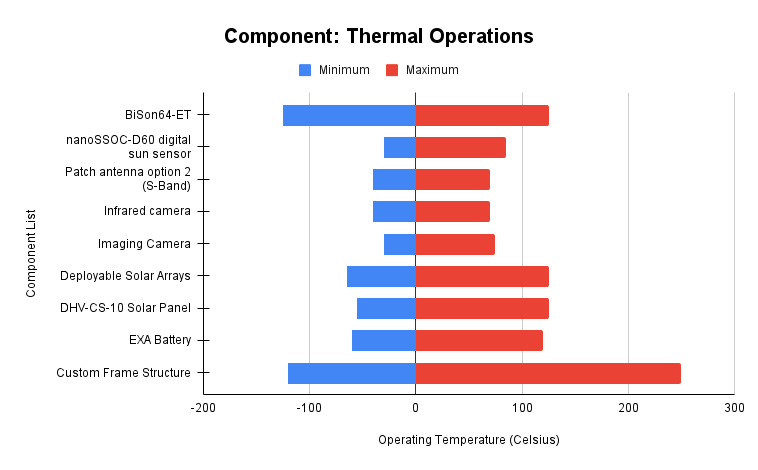
\includegraphics[width=\textwidth,frame, height=8cm]{Images/thermal.png}
    \caption{Thermal Limitations}
    \label{fig:thermal}
\end{figure}
\newpage
\subsection{Propulsion }
The general analysis conducted to identify a comprehensive list of propulsion methodologies involves identifying the set of maneuvers necessary to reach orbit altitude and adjust the inclination when necessary. Primary propulsion technologies would be used for orbit adjustment including shaping, changing, and maintaining altitude before and after reaching target orbit. Optimizing the orbit will determine the rate of propellant use and how long it can maintain its orbit, and by extension its lifetime. To reduce the consumption of propellant and the need for high powered propulsion systems, unnecessary and costly maneuvers must be avoided. Inclination change is one such reason; that requires significant propellant and thruster firings to manage. STK and python scripts were utilized to estimate the required total-Impulse for the Hohmann transfer from the departure orbit of CubeSat at an altitude of 400 km to the designated orbit of 800 km at a similar inclination of 35$^0$.
\begin{figure}
    \centering
    \subfloat[ $\Delta V$ vs S/C Mass propulsion]{{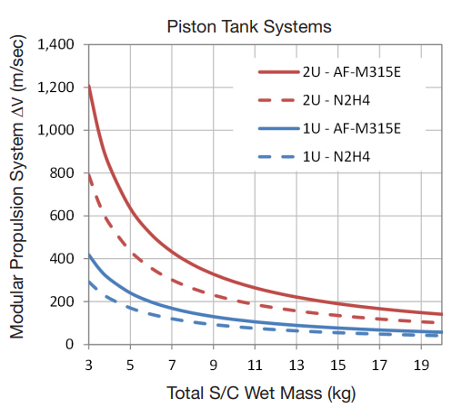
\includegraphics[width=7cm]{Images/p1.png} }}\label{fig:p1}
    \qquad
    \subfloat[Propulsion Tank ]{{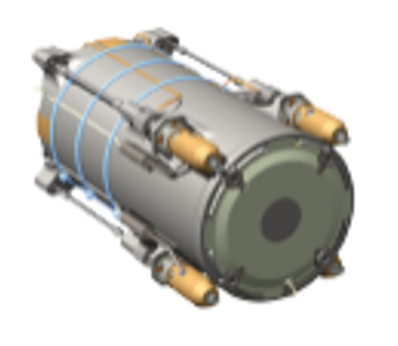
\includegraphics[width=7cm]{Images/p2.png} }}\label{fig:p2}
    \caption{Aerojet Rocketdyne Piston Tank Modular Propulsion System}
    \label{fig:prop}
\end{figure}

The maneuver to change altitude is conducted with a green monopropellant propulsion systems produced by Aerojet Rocketdyne \cite{Vacco}. The total Impulse managed by this propulsion system using an AF-M315E propellant blend for better performance and safety is sufficient for the maneuver with an estimated Delta V of 400 m/s for the wet mass of the designed CubeSat (See Figure (\ref{fig:prop})a). The MPS-130-2U piston \cite{SatCatalog} fed modular propulsion system utilizes a non-toxic green monopropellant delivering up to a 50\%  increase in density specific impulse while having a reduced footprint compared to similar velocity impulse systems operated with Hydrazine (Table \ref{Tab:Prop}). Green Monopropellant (highlighted red in the table) is chosen because it reduces fire hazards, has less equipment overhead, and weighs less compared to Hydrazine based propulsion systems. \\

\begin{table}[!ht]
\centering
\caption{Propellant Comparison}
\begin{tabular}{l|c|l|c|l|c|}
\rowcolor[HTML]{C0C0C0} 
Propulsion System        & \multicolumn{2}{c}{MPS-130-2U} \\ \hline
Dimensions (cm)          & \multicolumn{2}{c}{10x10x20} \\
Thrust (N)               & \multicolumn{2}{c}{0.25 - 1.0}   \\ 
Propellant               & \cellcolor{red!20}Green Monopropellant (AF-M315E)   & Hydrazine\\ \hline
Dry Mass (kg)            & \cellcolor{red!20}1.4                               & 1.5  \\
Wet Mass (kg)            & \cellcolor{red!20}2.5                               & 2.8  \\
Estimated Delta V (m/s)  & \cellcolor{red!20}400                               & 300  \\ 
Total Impulse (N-s)      & \cellcolor{red!20}2720                              & 1960 \\ \hline
\end{tabular}
\label{Tab:Prop}
\end{table}

\subsection{Structure}
Structure configuration for any CubeSat requires a lightweight material capable of withstanding the environmental elements it would be exposed to such as aerodynamic, gravitational, and solar torques that could arise during liftoff and transonic periods. The prevalence of electronic components onboard requires as little interference as possible, as such a non-magnetic 7000 series Aluminum alloy is commonly utilized \cite{TheWorldMaterial2021}. These alloys are tempered through multiple processes such as solution heat-treated by homogenizing the 7075-alloy cast for several hours, quenching for stress relief, then artificially aged to stabilize the microstructure and meet process requirements. This process allows the materials to obtain desirable characteristics such as improved strength, low density, corrosion resistance, better crack, and fatigue resistance. The T651 alloy was found to have better overall mechanical properties as shown in Table \ref{Tab:alloy} and was the choice of material for the 6U casing design .

All structures have natural frequencies of vibration which create large amplitudes that can lead to fatigue failure, undesirable noises, and reduced performance. A modal analysis for the natural frequency and mode shape is therefore conducted on the designed casing structure (Figure \ref{fig:casing}) to understand how the model reacts to external disturbances in a free vibration simulation, where more than one node participates in the system response. This analysis helps identify peak frequencies at or near structure natural frequency that may affect the performance of the structure. A sample of this response at a peak frequency of 127.1 Hz has a maximum deformation of about 0.46 mm as shown in Figure \ref{fig:modal}. 
\\
\begin{table}[!ht]
\centering
\caption{Aluminum Alloy Comparison}
\begin{tabular}{lc|lc|lc}
\rowcolor[HTML]{C0C0C0} 
Aluminum Alloy                          & \cellcolor{red!20}Al7075-T651   & Al7075-T7351 \\ \hline
Yield Strength (MPa)                    & \cellcolor{red!20}505           & 435  \\
Ultimate Tensile Strength (MPa)         & \cellcolor{red!20}570            & 510  \\
Modulus of Elasticity (GPa)             & \cellcolor{red!20}72             & 70  \\
Brinell Hardness                        & \cellcolor{red!20}150            & 140  \\ \hline
Density (g/cc)           & \multicolumn{2}{c}{2.81} \\ 
Poisson's Ratio          & \multicolumn{2}{c}{0.32} \\
{Coefficient of Thermal Expansion @20-100$^o$C (\si{\micro}m/m$^o$C)}  & \multicolumn{2}{c}{23.4} \\
\end{tabular}
\label{Tab:alloy}
\end{table}
\\
\begin{figure}[hbt!]
    \centering
    \vspace{5mm}
    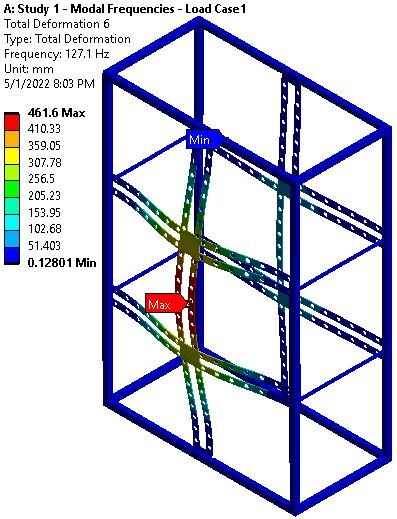
\includegraphics[width=\textwidth,height=7cm,
  keepaspectratio, scale=0.6]{Images/modal.JPG}
    \caption{Modal analysis of structure at peak frequency of 127.1 Hz}
    \label{fig:modal}
\end{figure}